\chapter{针对移动相机的快速视频背景减除技术}
 \label{ch4:FMCBS}
 本章对移动相机情况下的视频背景减除技术进行了研究,提出了一种针对移动相机的基于无参数模型的快速视频背景减除算法。该算法主要利用两方面的线索得到视频中准确的前景对象。首先引入最相似变形(as-similar-as-possible warping, ASAPW)方法对相机的运动进行估算和补偿,利用无参数的采样背景模型进行背景建模,利用背景模型这一前景外观线索获得粗略的前景结果。与目前已有的其他方法不同的是,本章所提出的算法不需要计算稠密光流或像素点轨迹等预处理过程,而是通过本章提出的基于超像素种子点的区域增长算法(superpixel-based seeded region growing, SSRG) 将基于稀疏光流的前景线索扩散到整幅图像范围,获得另外一个基于运动线索的粗略前景结果。最后通过基于超像素的MRF优化过程对两种线索得到的粗略结果进行优化,最终获得准确的前景。大量实验证明了本章所提出算法的有效性,与目前领先的算法相比本章算法可以得到与之相近的前景准确度;但在计算速度方面,本章所提出的算法要快得多。

 \section{研究背景}
 \label{ch4:sec:background}
视频背景减除技术,或移动目标检测技术,的目的是将视频图像序列中每帧图像当中的移动前景和背景部分分离。该技术已经广泛应用于视频监控、目标跟踪、动作识别等领域。此外,该技术通常作为其他计算机视觉和计算机图形学应用的预处理步骤。例如,在机器人的自主导航中,需要预先将摄像头拍摄的视频中的前景和背景部分分离,提取后续工作中需要用到的前景目标。早期的视频背景减除技术研究当中,一般假定相机在拍摄视频时是静止的。在这种假设下,区分视频中的前景和背景主要依靠检测像素的运动情况\cite{GMMPAMI,Barnich2011ViBe,pbas,vibe,subsenseTIP}, 文献\inlinecite{BouwmansOverview}对静止相机情况下的背景减除技术进行了很好的综述。\par

近些年来,随着移动计算平台的快速发展,类似于智能手机、手持摄像机、智能机器人等设备越来越普及。针对移动相机拍摄视频的背景减除技术变得越来越重要。与静止相机情况相比,针对移动相机的视频背景减除技术要更加困难。由于相机的运动,使得前景和背景像素都会产生运动,不再有一个参考点。因此区分相机运动和前景运动是移动相机情况下视频背景减除技术需要解决的主要问题之一。研究人员在最近几年提出了一系列新算法来提高移动相机情况下的视频背景减除的精度\cite{iccv2009,kwak2011Generalized,Cui2012,Multitransform,gbsuperpixel,SubspaceTracking},但是这些算法的速度却很慢,一般处理一帧图像需要几秒钟的时间,例如文献\inlinecite{kwak2011Generalized,gbsuperpixel,SubspaceTracking}中所提出的算法。由于算法速度过慢,限制了这些算法在实际应用中的应用范围。在文献 ~\inlinecite{5.8s}中,提出了一种移动相机拍摄视频前景对象检测实时算法。由于使用了简化后的模型,该算法速度非常快,甚至可以在智能手机上实现实时处理。但是该算法的检测准确度却与前文提到的领先的算法有较大差距。本章中,以设计一个针对移动相机的快速视频背景检测算法为目标,希望该算法简单高效,在达到与其他先进算法类似的准确度的同时能够有更快的处理速度。\par

为了检测移动相机拍摄视频中的移动对象,一般考虑两方面的线索,即运动相关的线索和外观相关的线索。对于运动相关的线索,主要的困难在于区分来自于相机的运动和移动前景引入的运动。在之前的研究工作当中,一般使用全局单应性矩阵(global homography)\cite{5.8s,LiuCVPR09} 或者基础矩阵(fundamental matrix) \cite{kwak2011Generalized,LimPRFloating}来估算相机的运动,但是根据极线几何理论 \cite{Multitransform},只有在相机运动不包含平移或者场景中所有点共面的情况下,才可以用一个全局的单应性矩阵来描述相邻帧图像中像素一对一的对应关系。然而在实际应用中,这两个假设几乎很难满足。在本章所提出的算法中,引入用于视频稳定技术\cite{Liu2009ASAP,Liu_2013ASAP} 的ASAPW方法来估算并补偿相机运动。与之前的其他方法相比,ASAPW通过图像不同区域的多个单应性矩阵来估算相机运动,使得算法在理论和实践上都更加鲁棒,可以处理任意情况下的相机运动。在本章算法中,基于文献~\inlinecite{Liu_2013ASAP}中的算法,提出了一个更加高效的运动估补偿方法。\par

大多数主流的视频背景减除算法都需要额外的预处理步骤来计算视频帧图像的稠密光流 \cite{Multitransform,gbsuperpixel}、点轨迹 \cite{iccv2009,Cui2012,SubspaceTracking}、 或者进行运动分割\cite{kwak2011Generalized}。这些预处理步骤本身的计算难度和计算量均较大。本章算法中没有使用计算量大的稠密光流,而是利用效率更高的稀疏光流获得稀疏的背景种子点。利用图像的连续性特点,通过SSRG算法将这些背景种子点扩散至整幅图像。\par

对于基于像素外观的线索,本章算法引入了与文献~\inlinecite{Barnich2011ViBe,pbas,subsenseTIP}类似的基于背景像素采样的无参数的背景模型。根据文献
 ~\inlinecite{CD2014}的报道,在静止相机视频背景减除算法准确率比较中,基于采样一致模型的背景减除算法要优于基于混合高斯模型(gaussian mixture model, GMM)的算法。据作者所知,基于采样一致模型的背景模型还没有被用于移动相机视频背景减除技术当中。主要的原因在于基于采样的模型对运动补偿的误差非常敏感。由于本章算法利用ASAPW来准确的补偿相机运动,使得可以使用基于采样模型的背景模型。在本章算法中,对文献~\inlinecite{subsenseTIP}中提出的背景模型进行了改进,使得其更加适用于移动相机情况。此外,本章算法中通过CUDA~\cite{CUDA}并行化将该背景模型在GPU上进行了实现,大大提高了计算速度。\par

 在本章提出算法的最后,在根据运动线索、外观线索得到的粗略结果以及前一帧结果的基础上建立基于超像素的MRF优化框架。每个超像素的最终标记(前景或者背景)可以通过图割算法\cite{graphcut04}求解能量最小化问题得到。实验结果显示本章提出的算法在处理速度更快的情况下达到了与其他先进算法类似的准确度。


综上所述,本章所提出的针对移动相机的视频背景减除快速算法的主要特点和优势在于:
\begin{enumerate}
\item 本章所提出的算法将现有的图像变形技术和基于采样的无参数背景模型方法结合到移动相机背景减除算法中;
\item 本章所提出的算法利用稀疏光流和SSRG来区分相机引起的运动以及前景引起的运动,相比于基于稠密光流和像素点轨迹的方法,本章所提出的方法速度更快但效果与之接近;
\item 通过GPU和CPU上的混合编程,本章算法处理大小为640$\times$480像素的视频速度可以达到8帧/秒,这是基于稠密光流的算法\cite{gbsuperpixel}的45倍。
\end{enumerate}


 \section{相关工作}
 \label{ch4:sec:relatedWorks}

 \subsection{静态相机视频背景减除}
 \label{ch4:sec:sub:scbs}

 文献~\inlinecite{Chien2002Efficient}提出了一种背景图像注册技术,用于建立可靠的背景图像。通过比较当前图像帧与所创建的背景图像可以获得前景结果。该算法假设相机是固定的,因此无法处理移动相机情况。文献~\inlinecite{Kim2001Moving}提出了一种用户交互的视频移动前景提取算法。该算法主要有帧内分割处理和帧间分割处理两部分组成。其中,帧内处理模块需要通过用户交互来定义那些用户感兴趣的语义对象,并且获得准确的对象边界。帧间处理模块则通过边界和区域跟踪来获得移动对象的准确边界信息。 Meier和 Ngan\cite{Meier1998Automatic} 提出了一种基于二进制图像模型的自动移动对象检测算法。该二进制模型可以通过图像的边缘信息提取,并在每帧图像进行更新。然而该算法提取前景结果的准确度对第一帧初始结果十分敏感。当第一帧初始结果不准确时,该算法的准确度会受到重要影响 \par
Barnich等人提出了一种基于无参数采样一致模型的背景减除算法,ViBe \cite{Barnich2011ViBe}。ViBe算法利用像素级的颜色空间采样值建立背景模型。该算法的背景模型比基于概率模型的算法\cite{GMMPAMI}更为简单,但是在前景检测准确度以及计算速度上却优于后者,特别是对于那些包含动态背景的视频中。 Hofmann等人对ViBe算法进行了改进,提出了PBAS算法。该算法通过定位不稳定区域并且以反馈的方式调整不稳定区域内模型的距离门限、更新率等参数使得算法的前景提取准确度进一步提高。随后,文献 \inlinecite{subsenseTIP}提出了一种基于更加有效的反馈式模型参数更新机制的算法,SuBSENSE。该算法中的背景模型中除了基于颜色空间采样值外还加入了特征空间的采样值。文献~\inlinecite{LBP06}中最早提出了基于纹理特征的背景减除算法,通过局部二进制模式(local binary pattern,LBP)对背景进行建模,相比颜色空间模型取得了更好的效果。在SuBSENSE算法 \cite{subsenseTIP}中使用了与LBP类似的局部二进制相似模式(local binary similarity pattern,LBSP)采样模型。相比于LBP,LBSP可以在多张相邻图像帧之间进行计算,具有时域相关性强的优势。在公开的视频背景减除测试数据库CD.Net 2012~\cite{CDNet2012}以及CD.Net 2014~\cite{CD2014}中,该算法的各项指标排名均名列前茅。但是由于该算法是针对静止相机的,并不能直接用于处理移动相机情况下的背景减除任务。\par

\subsection{移动相机视频背景减除}
\label{ch4:sec:sub:mcbs}
在之前的移动相机背景减除算法中,一般用单应性 矩阵或基础矩阵来估算相机的运动。在文献~\inlinecite{Multitransform}中,作者提出使用多变换模型来处理相机的运动。该算法根据相邻图像帧的几何关系从单应性矩阵模型和基础矩阵中选择一个合适的模型。当选择单应性矩阵模型时,可以通过一个全局一对一的矩阵建立相邻帧间像素之间的关系;而当选择基础矩阵时,由于基础矩阵无法建立图像间像素一对一的关系,因此只能在一系列单应性矩阵中选取均方误差最小的单应性矩阵来估算相机运动。 在这种情况下,虽然最后估算的单应性矩阵均方差最小,但是该矩阵仍然被应用到图像中每个像素。在相机运动不受约束的情况下,相邻帧图像像素之间无法通过单应性矩阵建立一对一的对应关系。在本章算法中,通过引入并改进ASAPW技术 \cite{Liu2009ASAP,Liu_2013ASAP}来估算并补偿相机运动。本章算法在变形能量方程中使用更简单的数据项,并且提出一种更加有效的动态参数设置方法自适应调整各个单元的形状保持权重系数。 \par

文献~\inlinecite{kwak2011Generalized}使用贝叶斯滤波框架来估算视频帧图像中像素的运动以及外观变化模型,提出了一种通用的移动相机视频背景减除算法。该算法需要在第一帧获得较高准确度的前景分割结果,并在随后的图像帧中对前景进行可靠跟踪。因此文献~\inlinecite{kwak2011Generalized}的算法无法处理那些包含复杂运动的长视频。文献~\inlinecite{gbsuperpixel}提出了一种基于超像素概率密度估计的视频背景减除算法,该算法建立超像素级别的运动模型和外观模型,并通过二进制置信传播(binary belief propagation)获得像素级别的前景检测结果。由于算法复杂度较高,该算法处理一帧图像需要6秒。\par

另一类针对移动相机的视频背景减除算法依靠像素点轨迹信息来估算视频中的前景。文献~\inlinecite{iccv2009}提出了一种基于滑动窗口的像素点轨迹矩阵分解的算法。该算法使用RANSAC\cite{Ransac}算法估计背景像素点轨迹。文献~\inlinecite{Cui2012}提出一种将点轨迹矩阵分解为低秩部分(背景)和群稀疏部分(前景)。文献~\inlinecite{SubspaceTracking}提出一种基于像素点轨迹的在线背景建模方法,该方法通过跟踪描述背景运动的线性子空间建立背景模型。 在效率方面,文献~\inlinecite{SubspaceTracking}中算法需要1.8秒左右时间处理Hopkins数据集\cite{HopKinsDataSet} 中的一帧图像。\par

与上述方法不同,Yilmaz等人~\cite{contourTracking04}提出了一种基于轮廓(contour)的移动相机拍摄视频前景跟踪方法。通过主动轮廓模型(active contours)\cite{Snakes}可以对视频和图像中的前景进行跟踪。主动轮廓模型的目标是获得紧密包围对象的轮廓,一般通过能量最小化的方式实现。文献~\inlinecite{contourTracking04}将能量函数定义为:
$$ E(\Gamma) = \int_{0}^{1} E_{image}(\mathbf{v})+ E_{shape}(\mathbf{v}) ds,$$
其中,$E_{image}$为根据图像本身的颜色和纹理分布,$E_{shape}$则基于轮廓跟踪的历史数据,保证在前景被遮挡的情况下保持对象的形状。该算法可以在不需要估算相机运动的情况下对移动相机拍摄视频中的前景对象进行可靠跟踪,而且能处理前景被遮挡的情况。但是由于是基于轮廓跟踪的方法,容易受到背景区域中边缘等结构信息的干扰。此外基于变分的方法求解时需要多次迭代,造成算法比较耗时。

 \section{算法描述}
 \label{ch4:sec:algorithm}
 本章提出算法的流程流程图如图~\ref{ch4:fig:1}所示。首先,利用文献~\inlinecite{superpixel}的算法将输入视频图像帧分割为若干超像素;随后使用KLT算法~\cite{KLT}计算每个超像素中心点的稀疏光流;通过ASAPW来估算相机运动情况,将每个超像素光流与估算的相机运动进行比较,获得若干稀疏的背景种子点;利用SSRG算法将这些稀疏运动线索扩散到整幅图像,得到一个基于运动线索的粗略前景分割结果。另一方面,利用ASAPW算法估算的相机运动对输入视频帧图像进行运动补偿,并将补偿后的图像帧与非参数的背景模型进行比较,从中可以得到另一个基于外观模型的粗略前景结果。最后,通过基于超像素的时域相关MRF优化过程来对基于运动线索和基于外观线索的两个粗略前景分割结果进行优化,通过图割算法\cite{graphcut04}求解能量最小化问题得到每个超像素最终的前景分割结果。

\begin{figure}[!htbp]
\begin{center}
\begin{tabular}{c}
% Use the relevant command to insert your figure file.
% For example, with the graphicx package use
  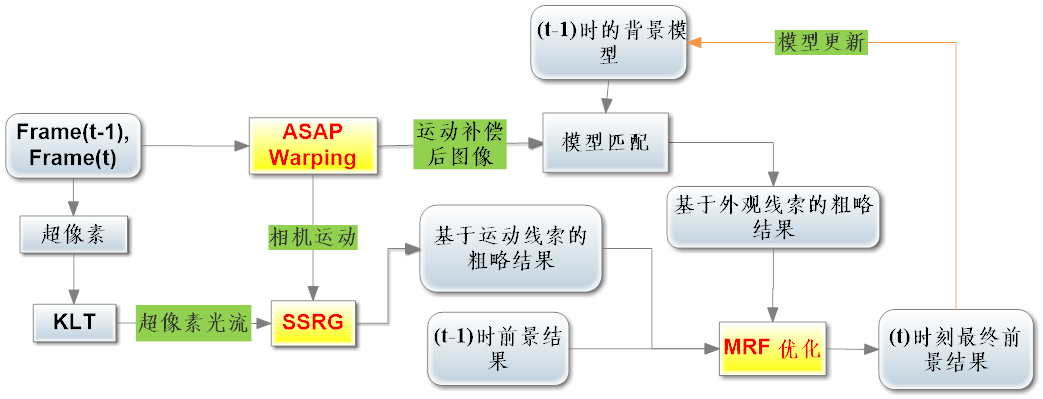
\includegraphics[width=0.9\textwidth]{ch4/FlowchartSmallChs.png}
  \end{tabular}
% figure caption is below the figure
\end{center}
\caption{算法流程示意图,主要部分用黄色标记}
\label{ch4:fig:1}       % Give a unique label
\end{figure}


\subsection{基于ASAPW的相机运动补偿}
\label{ch4:sec:sub:asap}
文献~\inlinecite{Liu_2013ASAP}提出了一种用于视频稳定的基于变形的相邻帧图像运动补偿算法。如图~\ref{ch4:fig:2}所示,该算法将每一帧图像划分为均匀网格。相邻图像帧中的一对特征点\(p\) 和 $\hat{p}$ 分别位于网格 \(i\) 和 \(j\)当中。网格$i$和$j$的四个顶点分别为${V}_{p}=[{v}^{1}_{p}$,${v}^{2}_{p}$,${v}^{3}_{p}$,${v}^{4}_{p}]$, ${\hat{V}_{p}}=[\hat{v}^{1}_{p}$,$\hat{v}^{2}_{p}$,$\hat{v}^{3}_{p}$,$\hat{v}^{4}_{p}]$。因此,\(p\) 可以用网格\(i\)的四个顶点坐标的双线性插值表示:$p=\sum_{p}{{V}_{p}{w}_{p}}$。

 \begin{figure}[!htbp]
\begin{center}
% Use the relevant command to insert your figure file.
% For example, with the graphicx package use
  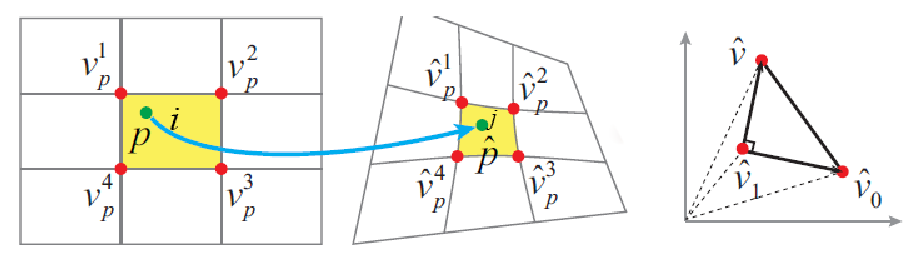
\includegraphics[width=0.75\textwidth]{ch4/asapN.eps}
  \par \quad\quad\quad(a)\quad\quad\quad\quad\quad\quad\quad\quad\quad\quad\quad\quad(b)
% figure caption is below the figure

\end{center}

\caption{ASAPW 示意图~\cite{Liu_2013ASAP}}
\label{ch4:fig:2}       % Give a unique label
\end{figure}
为了补偿相机运动,通过图像变形对当前帧图像进行变换,具体的变形通过求解能量最小化问题实现。
\begin{equation}\label{ch4:equ:asap}
  E(\hat{V}) = {E}_d(\hat{V}) + \alpha{E}_{s}(\hat{V})
\end{equation}
其中$E_d$为数据项,定义为:
\begin{equation}\label{ch4:equ:dataterm}
  {E}_{d}(\hat{V}) = \sum_{p}{\parallel\hat{V}_{p}{w}_{p}- \hat{p}\parallel}^{2}
\end{equation}
主要作用是保证 \(p\) 与 $\hat{p}$可以用相同的基于网格顶点的双线性插值表示。 公式~\ref{ch4:equ:asap}中$E_s$为平滑项,具体定义为:
$${E}_{s}(\hat{V} )= \sum_{\hat{v}}\parallel\hat{v}-\hat{v}_{1} - s{R}_{90}(\hat{v}_{0} - \hat{v}_{1})\parallel^{2}, s=\frac{\parallel{v}-{v}_{1}\parallel}{\parallel{v}_{0}-{v}_{1}\parallel},{R}_{90} = \left(\begin{array}{cc}{0} &{1} \\{-1} &{0}\end{array}\right),$$
主要作用是保证变形后的图像中相邻三角形的变换为相似变换,保持图像的形状不变。
公式~\ref{ch4:equ:asap}中的$\alpha$为权重因子,调整数据项和平滑项之间的权重比值。由于公式~\ref{ch4:equ:asap}中的方程是一个线性方程组,变形后的网格角点坐标$\hat{Vp}$可以通过求解稀疏线性方程组得到。对于每个网格,利用网格的四个顶点可以得到一个单应性矩阵。整幅图像的运动可以通过这些二维网格上的一系列单应性矩阵表示。与基于全局单应性矩阵的其他运动估计算法相比,ASAPW的效果要更好~\cite{Liu_2013ASAP}。 \par
从图~\ref{ch4:equ:dataterm}可以看出,随着匹配特征点数量的增加,数据项所包含的约束会随着线性增长。当匹配的特征点数太多时,会造成求解大规模稀疏线性方程组的速度变慢,从而影响整个算法的效率。基于此原因,本章算法提出利用网格内特征点直接估算网格内单应性矩阵,从而得到网格顶点变形后坐标。对于网格内包含足够特征点以估算网格内单应性矩阵的网格,将其标记为$h$,他们的数据项定义为:

 $$E^{h}_{d}(\hat{V}) = \sum_{p\in h}{\parallel H_{p}V_{p} - \hat{V_{p}}\parallel}^2$$
其中 $H_{p}$ 为包含$p$的顶点的网格单元的单应性矩阵。估算8个自由度的$3\times3$ 单应性矩阵最少需要4组对应的特征点,为了使估算更为准确,在本章算法中最少选取10组特征点来估算网格内的单应性矩阵。对于那些少于10组特征点的网格,无法估算网格内单应性矩阵,对于这些网格使用基于公式~\ref{ch4:equ:dataterm}的双线性插值约束数据项。最终,本章的图像变形算法的数据项定义为:
$${E}_{d}(\hat{V}) = \sum_{p \notin h}{\parallel\hat{V}_{p}{w}_{p}- \hat{p}\parallel}^{2} +
\sum_{p\in h}{\parallel {H_{p}V_{p} - \hat{V_{p}}}\parallel}^2.$$
为了选择合适的权重因子$\alpha$,文献~\inlinecite{Liu_2013ASAP}中将$\alpha$ 均匀分为十个0.3至3之间的离散候选值。计算这十个候选值的变形误差,最终选择变形误差最小的值作为权重因子。该方法需要重复计算图像的变形误差,效率较低。本章算法对其进行了改进,通过自适应调整的方式来设置每个网格内的权重因子,通过网格$c \in h$内的变形误差$e_{c} = {\parallel H_{c}p_{c} - \hat{p_{c}} \parallel}^2 $,设置权重因子值为:
 $$ \alpha_{c\in h} = s_{1}\exp({e_{c}/avgErr})+ s_{2} $$
 其中$s_{1}$ 为常数固定值0.15, $avgErr$ 为$h$的平均变形误差, $s_{2}$ 为截断因子使得 $\alpha_{h} \in [0.3,3.0]$。对于那些特征点数小于10的网格,其权重因子设定为固定值, $\alpha_{c \notin h} = 1.0$。通过这种方式,使得那些变形误差较小的网格的数据项获得更大的权重,而那些误差大或者不包含特征点的纹理平滑区域则更多依靠相似变换来保证变形的准确度。
\subsection{基于超像素种子点的区域增长算法}
\label{ch4:sec:sub:ssrg}
由于准确的图像逐像素稠密光流的计算量非常大,本章算法提出通过基于KLT算法~\cite{KLT}的稀疏光流以及超像素种子点区域增长算法(SSRG)来得到前景的粗略分割结果。由于像素级的相机运动已经通过~\ref{ch4:sec:sub:asap}节中介绍的ASAPW得到,因此可以计算每个超像素内像素的平均运动得到超像素级的相机运动估算结果。将此相机运动与基于超像素的光流进行比较,可以得到前景线索。在理想情况下,由于背景区域像素的运动是由于相机运动产生的,因此其光流应该与相机运动一致。如果某超像素的光流与相机运动的差距小于某阈值,在本章算法中使用较小的阈值0.4,那么该超像素被标记为背景种子点。利用图像像素在空间域和颜色空间分布的连续性,相邻及相似的像素同属于背景或同属于前景的几率较大,本章提出利用SSRG算法将稀疏的背景种子点扩散到整幅图像,见算法~\ref{ch4:alg:ssrg}。本章提出的SSRG算法与文献~\inlinecite{seededRegionGrowing}相似,但是主要有以下两个区别: (1) 本章所提出的SSRG算法与文献~\inlinecite{seededRegionGrowing}的目的不同,前者目的是将图像分割为前景区域和背景区域两个部分,而后者则是将图像分为多个齐次区域;(2)本章提出的SSRG算法基于超像素,在效率上比文献~\inlinecite{seededRegionGrowing}中基于像素的算法更具优势。

\renewcommand{\algorithmcfname}{算法}
\begin{algorithm}
\caption{基于超像素种子点的区域增长算法}
\label{ch4:alg:ssrg}
\LinesNumbered
\KwData {图像 $I$ 的超像素$superpxiels$ , 背景种子点集合 $seeds$, 区域增长门限$threshold_{rg}$ }
\KwResult {背景结果 $mask$}
 $\forall p \in superpixels$, $mask[p] \leftarrow 0$ , $segmented[p] \leftarrow 0$ \;
\ForEach {$s$ in $seeds$}{
  $mask[s] \leftarrow 1$ \;
 {$regColor \leftarrow  Color(s)$ \;}
 {$dist \leftarrow 0 ,  regSize \leftarrow 1$ \;}
 {清空$list$ \;}
\While {$dist < threshold_{rg}$ 且 $regSize < \sharp Superpixels$}{
\ForEach {$p \in $ Neighbors of $s$}{
\If{ $!segmented[p]$ and $p \notin list $}{
 { 将$p$ 添加到 $list$ \;}
}
}
 $\hat{m} \leftarrow  \arg\min_{m \in list}{\parallel regColor - Color(m) \parallel}$ \;
 $  mask[\hat{m}] \leftarrow 1, segmented[\hat{m}] \leftarrow 1$ \;
 $dist \leftarrow \parallel regColor - {Color(\hat{m})} \parallel $ \;
 $regColor = \frac {regColor \times regSize + Color(\hat{m})}  {regSize + 1 }$ \;
 $regSize \leftarrow regSize$ $+ 1$ \;
从 $list$ 中删除 $\hat{m}$\;
\If {$list$ 为空}{
 跳出循环\;
}
}
}

\end{algorithm}

算法~\ref{ch4:alg:ssrg}的一个计算实例如图~\ref{ch4:fig:3}所示。图~\ref{ch4:fig:3}中(a)和(b)分别为文献~\inlinecite{HopKinsDataSet}数据库中Car4视频的第41和42帧图像的超像素分割结果。图~\ref{ch4:fig:3}(c)为背景超像素种子点,用白色标识,本章SSRG算法的输出结果见图~\ref{ch4:fig:3}(d)。从图中可以看出,通过SSRG算法可以有效的将稀疏的背景种子点扩散到前景对象除外的整幅图像,图~\ref{ch4:fig:3}(d)中黑色区域大部分为前景对象,有少部分为图像的边界或连续性差的背景区域。图~\ref{ch4:fig:3}(d)中得到的前景结果精度还比较低,仍需进一步进行优化处理。
% For one-column wide figures use
\begin{figure}[!htbp]
\begin{center}
% Use the relevant command to insert your figure file.
% For example, with the graphicx package use
 % \includegraphics[width=0.25\textwidth]{lsuperpixel.png}\quad
%  \includegraphics[width=0.25\textwidth]{superpixel.png}\quad
%  \includegraphics[width=0.25\textwidth]{seeds.png}\quad
%  \includegraphics[width=0.25\textwidth]{motionCue.png}\\
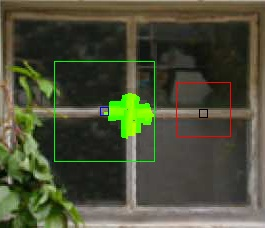
\includegraphics[width=1.0\textwidth]{ch4/fig3.eps}\\
  (a)\quad\quad\quad\quad\quad\quad\quad\quad(b)\quad\quad\quad\quad\quad\quad\quad\quad(c)\quad\quad\quad\quad\quad\quad\quad\quad(d)
% figure caption is below the figure
\end{center}

\caption{SSRG算法执行结果示例。 (a) $frame_{t-1}$超像素分割, (b) $frame_{t}$超像素分割 , (c) 背景中子点, (d) SSRG算法结果。}
\label{ch4:fig:3}       % Give a unique label
\end{figure}

\subsection{基于采样一致的背景模型}
\label {ch4:sec:sub:scam}

本章算法通过对每个像素点在色彩空间和LBSP的多个采样值来建立背景模型~\cite{subsenseTIP}。假设图像$I$中的某像素$I(x)$的背景采样点模型为$B(x)$,根据文献~\inlinecite{subsenseTIP}的定义,$B(x)$的大小为50,即通过50个采样点来描述每个像素的背景模型。在模型匹配阶段,图像中每个像素的颜色和LBSP值与$B(x)$中的各个采样值进行比较。如果$I(x)$与某个采样值$B(x)[i]$之间的距离在某个门限 $T(x)$之内,那么$B(x)[i]$则被称为匹配采样点。假如匹配采样点的个数大于匹配门限 $ T_{n}$,则像素 $I(x)$ 被标记为背景像素,反之则被标记为前景像素。在计算过程中$T_{n}$ 为固定常数2,$T(x)$则是像素级的门限变量控制匹配采样点与背景点之间的最大距离。在文献~\inlinecite{pbas,subsenseTIP}所提算法中,通过一种反馈机制来动态自适应调整$T(x)$,其中颜色空间和LBSP特征点空间的门限值分别由一个像素级变量$R(x)$控制:


$$T_{color}(x) = R(x) \cdot R^{0}_{color},$$
$$T_{lbsp}(x) = 2^{R(x)} + R^{0}_{lbsp},$$
其中 $R^{0}_{color}$ 和 $R^{0}_{lbsp}$ 为颜色空间和LBSP特征空间的最小距离门限,分别为固定值30和3\cite{subsenseTIP}。在本章所提出的算法中,通过反馈机制对$R(x)$的值进行动态更新:

$$ R(x) = \begin{cases}  R(x)+v & if \quad {R(x)<(1+2D_{min}(x))}^{2} \\  R(x) - \frac{1 }{v } & otherwise \end{cases}$$
其中 $D_{min}(x)$ 为采样模型$B(x)$ 与 $I(x)$间归一化的最小距离。与文献~\inlinecite{subsenseTIP}算法不同的是, 在文献~\inlinecite{subsenseTIP}算法中$v$ 值也会根据前景结果的闪烁情况进行动态更新,而本章算法对此进行了简化,将$v$的值设置为固定常数0.1。主要的原因在于,在移动相机情况下,受到运动补偿的准确性影响,前景结果的闪烁情况(即某像素时而被标记为前景,时而被标记为背景,出现闪烁现象)比较难跟踪。此外,在移动相机情况下,模型的更新率应该比静止相机情况更快,以减少相机补偿的累积误差。在本章所提的算法中,通过最终的前景/背景标记结果对背景采样模型进行更新。文献~\inlinecite{subsenseTIP}算法中模型更新率同样是一个动态变化的像素级变量,为了提高效率本章算法将其进行了简化。对于标记为背景的像素$I_{B}(x)$,用$I_{B}(x)$ 其随机邻域像素更新$I_{B}(x)$中 $10\%$的采样点;对于标记为前景的像素,只以$50\% $ 的 概率更新一个采样点。改进后的更新模式更加简单且适用于移动相机情况。 \par
由于采样模型对各个像素是相互独立的,因此可以通过并行编程的方式实现。本章算法将背景模型通过CUDA~\cite{CUDA}在GPU上进行了实现。对于每个像素$I(x)$,单独启动一个线程来将其与背景模型$B(x)$进行比较。随后,在此线程中进行$R(x)$和 $T(x)$等参数的更新。当通过MRF优化过程得到最终的前景结果时,对每个像素启动一个线程来对采样模型$B(x)$进行更新。

\subsection{基于超像素的MRF优化}
\label {ch4:sec:MRF}

通过~\ref{ch4:sec:sub:ssrg}节和~\ref{ch4:sec:sub:scam}节介绍的方法,可以分别得到基于运动线索和基于外观线索的粗略前景分割结果。但由于这两个粗略结果的精度均不高,需要进行进一步优化处理。本章算法提出一种基于超像素的MRF优化框架。本章的MRF优化框架受到了静态相机视频背景减除优化算法~\cite{MRF}的启发,假设${F}_{t}$ 为$t$ 时刻输入视频图像帧${I}_{t}$的前景,$S_{t}$为图像的超像素分割结果,${{F}_{t}}^{M}$为基于运动线索的粗略前景分割结果,${F_{t}}^{A}$ 为基于外观线索的粗略前景分割结果。此外,根据视频的连续性,在前一帧中为前景对象的像素,在后续图像帧中是前景的概率较大。本章的优化算法的目标是通过${{F}_{t}}^{M}$、${{F}_{t}}^{A}$以及上一帧图像的前景结果得到优化后的最终前景结果 $F_{t}$。根据文献~\inlinecite{MRF}定义的超像素前景概率,超像素$s$ 属于前景的概率为:
\begin{equation}
\label{ch4:equ:fgprop}
\hat{P_{t}(s)} = \frac{c\sum_{x \in s}{F_{t}}^{A}(x) + (1-c)\sum_{x \in s}{F_{t}}^{M}(x)}{\vert s \vert}
\end{equation}



 其中 $c$ 为外观背景模型的可信度权重因子, $\vert\cdot\vert$ 表示计算超像素的像素数。为了提高前景检测灵敏度,本章算法通过线性映射的方式定义最终超像素前景概率为 :
$$P_{t}(s) = \min(\theta \cdot \hat{P_{t}(s)},1)$$
其中 $\theta$ 为固定常数值 $2.0$。 参考文献 \inlinecite{graphcut04}的方式,结合图像空间域、时间域以及超像素前景概率,本章算法定义如下的能量函数:
\begin{equation}
\label{ch4:equ:mrf}
E(F_{t}(S)) = \lambda_{1}\sum_{s \in S_{t}}{U(F_{t}(s))} + \lambda_{2}\sum_{(s_{t}(i),s_{t}(j))\in N}{V(F_{t}(i),F_{t}(j))} + \lambda_{3}\sum_{s \in S_{t}}{T(F_{t}(s))}
\end{equation}



公式~\ref{ch4:equ:mrf}中的第一项为数据项,定义为:

$$ U(F_{t}(s)) = -\ln(P_{t}(s))F_{t}(s) - \ln(1-P_{t}(s))(1-F_{t}(s)), $$
公式~\ref{ch4:equ:mrf}中的第二项为空间相关性约束项:
\begin{equation}
\label{ch4:equ:mrfSpace}
V(F_{t}(i),F_{t}(j)) = \delta( F_{t}(i) - F_{t}(j)) (v_{1} + v_{2}\cdot e^{(-\frac{\parallel \mu_{t}(i) - \mu_{t}(j)\parallel}{2\beta})})
\end{equation}

其中$\delta()$ 为Kronecker delta函数, $\mu_{t}(s)$ 为 $t$时刻超像素 $s$的平均颜色,$\beta$ 为图像相关的变量,表示图像相邻超像素之间颜色距离的平均值, $v_{1}$ 和$v_{2}$ 为两个预先定义的常数,分别为 0.3 和 40。\par
公式~\ref{ch4:equ:mrf}中的最后一项为时间连续约束项。前景对象在视频的两个相邻图像帧中应该是连续的,假如某超像素在前一帧被识别为前景像素,那么该超像素在当前图像帧中的对应超像素有很大的概率也同样属于前景。本章算法利用超像素光流建立相邻图像帧超像素之间的关联。假设超像素$S_{t}(s)$的中心点为 $C_{t}(s)$。其在前一帧图像中的对应点$C_{t-1}(s)$可以通过超像素光流得到。超像素$S_{t}(s)$在前一帧图像中对应的超像素$\hat{S_{t-1}}(s)$定义为:
$$ \hat{S_{t-1}}(s) = \arg\min_{i\in S_{t-1}}(\alpha_{s}\parallel (C_{t-1}(s) - C_{t-1}(i))\parallel + (1-\alpha_{s})\parallel \mu_{t-1}(i) - \mu_{t}(s)\parallel) $$
其中 $\alpha_{s} $ 为控制空间距离可靠性的权重因子,本章算法中将其设为固定值0.9。因此,公式~\ref{ch4:equ:mrf}中的最后一项具体定义为
$$ T(f_{t}(s)) = v_{3}(1-\delta(F_{t}(s)-F_{t-1}(\hat{S_{t-1}}(s))))\cdot e^{-\frac {\parallel \mu_{t}(s) -\mu_{t-1}(\hat{S_{t-1}}(s)) \parallel}{2\beta}}$$
其中 $v_{3}$ 为线性映射函数使得公式~\ref{ch4:equ:mrf}中的三项值的大小相互接近。在本章算法中, $v_{3}$以及公式~\ref{ch4:equ:mrfSpace}的值设置为固定值40。\par



% For one-column wide figures use
\begin{figure}[htbp]
\begin{center}
% Use the relevant command to insert your figure file.
% For example, with the graphicx package use
  %\includegraphics[width=0.18\textwidth]{modelCue.png}
%  \includegraphics[width=0.18\textwidth]{imotionCue.png}
%  \includegraphics[width=0.18\textwidth]{lastMask.png}
%  \includegraphics[width=0.18\textwidth]{currMask.png}
%  \includegraphics[width=0.18\textwidth]{groundtruth.png}
   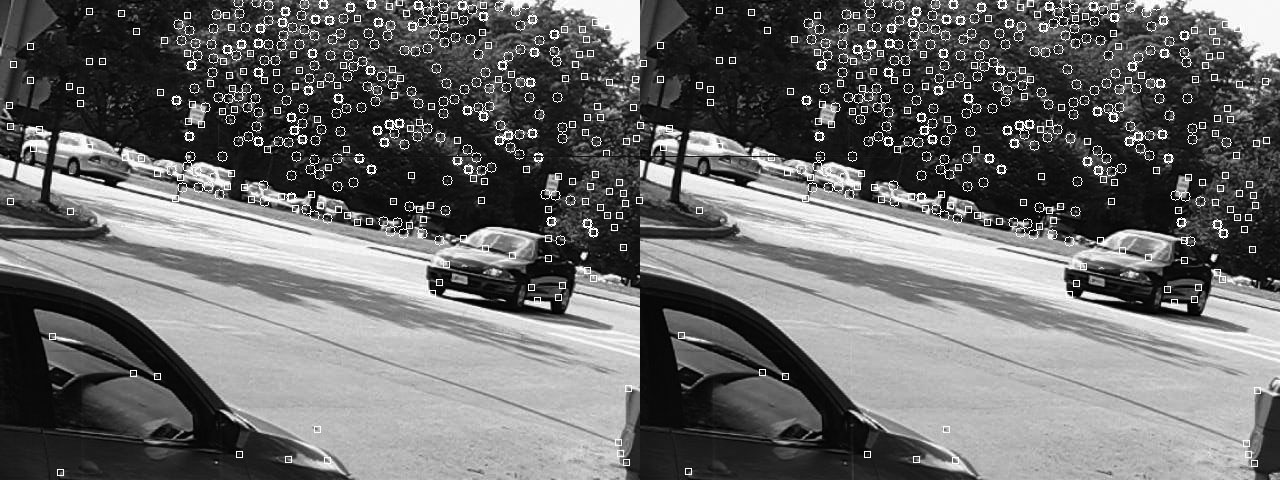
\includegraphics[width=1.0\textwidth]{ch4/fig4.eps}\\
(a)\quad\quad\quad\quad\quad\quad(b)\quad\quad\quad\quad\quad\quad(c)\quad\quad\quad\quad\quad\quad(d)\quad\quad\quad\quad\quad\quad(e)
% figure caption is below the figure
\end{center}

\caption{MRF 优化过程示意图,(a)基于外观模型的粗略前景结果, (b)基于运动线索的粗略前景结果, (c) 上一帧图像前景结果, (d) 优化后结果, (e) 正确结果}
\label{ch4:fig:mrf}       % Give a unique label
\end{figure}

最后,视频中的背景减除问题可以转换为能量最小化问题,即寻找 $F_{t}(S)$ 使得公式~\ref{ch4:equ:mrf}中的能量值 $E(F_{t}(S))$ 最小。能量方程求最小值可以通过高效的图割算法\cite{graphcut04}实现。图~\ref{ch4:fig:mrf}中给出了本章提出的MRF优化方法的一个计算实例。其中图~\ref{ch4:fig:mrf}(a)和(b)分别为基于运动线索和基于外观背景模型的粗略前景分割结果,图~\ref{ch4:fig:mrf}(c)中为视频中前一帧图像的前景结果,图~\ref{ch4:fig:mrf}(d)为本章提出的MRF优化方法得到的优化后结果。从图~\ref{ch4:fig:mrf}(d)中可以看到,优化后的前景结果的准确度明显好于输入的两个粗略结果,证明了本章提出的基于超像素的MRF优化方法的有效性。由于本章算法MRF能量方程是在超像素上建立的,与基于像素的方法\cite{Multitransform,SubspaceTracking}相比,本章所提出的算法在计算速度上具有较大优势。为了保证提取前景的精度,在本章算法中超像素大小相对较小,每个超像素大约包含25个像素。 \par


 \section{实验结果与分析}
 \label{ch4:sec:results}
 \subsection{实验一}
 \label{ch4:sec:sub:test1}

为了测试本章提出算法的有效性,在Hopkins视频数据集\cite{HopKinsDataSet}中的(cars1-8, people1-2)视频、文献~\inlinecite{ParticleCVPR06}中的 (vcar, vperson)等视频上对本章提出的算法进行了测试。目前还没有一个针对移动相机拍摄视频背景减除算法的测试数据库,但是大部分研究移动相机视频背景减除技术的论文均在上述视频上进行了实验\cite{iccv2009,LimPRFloating,Multitransform,kwak2011Generalized}。由于Hopkins视频数据集并没有提供每一帧图像的正确前景结果,在实验前通过人工的方式提取每一帧中的准确前景用于算法准确性评估。\par
在本章的实验中,根据实验中视频大小以及文献~\cite{Liu_2013ASAP}的建议,在ASAPW过程中将输入图像帧分为 $8\times8$ 的均匀网格。算法~\ref{ch4:alg:ssrg}中的区域增长门限 $threshold_{rg}$ 的值设置为每帧图像中相邻超像素颜色距离的平均值。公式~\ref{ch4:equ:mrf}中的权重参数设置为$\lambda_{1} = 0.5, \lambda_{2} = 0.35, \lambda_{3} = 0.15$。公式~\ref{ch4:equ:fgprop}中的可信度权重因子$c$ 设置为$0.75$。在所有视频的测试中均使用同样的参数配置。 \par
在图~\ref{ch4:fig:result}中,给出了本章算法在部分视频图像中的测试结果以及与当前领先的算法\cite{kwak2011Generalized,Multitransform,5.8s}的比较。其中图~\ref{ch4:fig:result}的第一行分别为为cars2视频的第20帧图像,cars3视频的第19帧图像, cars4视频的第40帧图像,people1视频的第40帧图像以及people2视频的第16帧图像。图~\ref{ch4:fig:result}的第二行为正确的前景结果,图~\ref{ch4:fig:result}的第三至第六行为文献~\inlinecite{Multitransform},文献~\inlinecite{kwak2011Generalized},文献~\inlinecite{5.8s}中算法的结果以及本章算法的结果,其中用暗色表示算法检测出的背景区域,前景区域保持原来的颜色。

\begin{figure}[htb]
\begin{center}
% Use the relevant command to insert your figure file.
% For example, with the graphicx package use
  %\includegraphics[width=0.15\textwidth]{c2.png}
%  \includegraphics[width=0.15\textwidth]{c3.png}
%  \includegraphics[width=0.15\textwidth]{c4.png}
%  \includegraphics[width=0.15\textwidth]{p1.png}
%  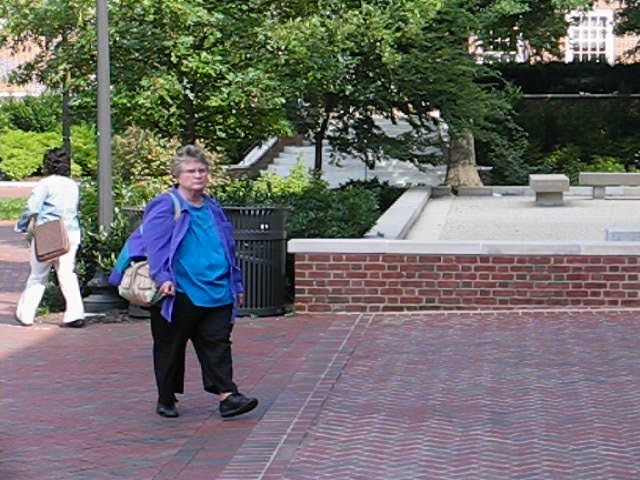
\includegraphics[width=0.15\textwidth]{p2.png}\\
%  \includegraphics[width=0.15\textwidth]{gtc2.png}
%  \includegraphics[width=0.15\textwidth]{gtc3.png}
%  \includegraphics[width=0.15\textwidth]{gtc4.png}
%  \includegraphics[width=0.15\textwidth]{gtp1.png}
%  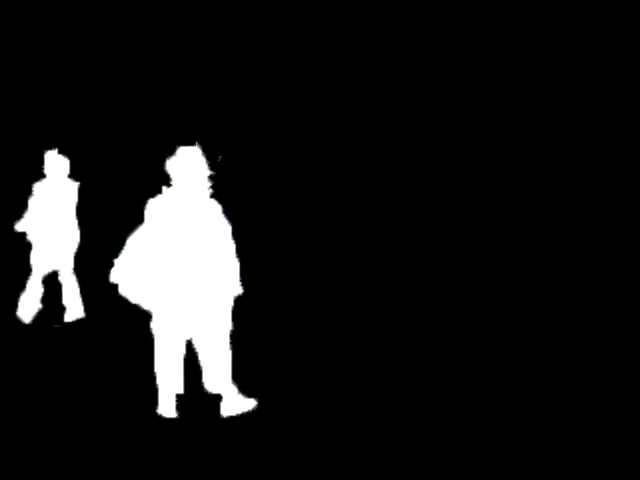
\includegraphics[width=0.15\textwidth]{gtp2.png}\\
%  \includegraphics[width=0.15\textwidth]{c2_m.png}
%  \includegraphics[width=0.15\textwidth]{c3_m.png}
%  \includegraphics[width=0.15\textwidth]{c4_m.png}
%  \includegraphics[width=0.15\textwidth]{p1_m.png}
%  \includegraphics[width=0.15\textwidth]{p2_m.png}\\
%  \includegraphics[width=0.15\textwidth]{c2_k.png}
%  \includegraphics[width=0.15\textwidth]{c3_k.png}
%  \includegraphics[width=0.15\textwidth]{c4_k.png}
%  \includegraphics[width=0.15\textwidth]{p1_k.png}
%  \includegraphics[width=0.15\textwidth]{p2_k.png}\\
%  \includegraphics[width=0.15\textwidth]{c2_mcd.png}
%  \includegraphics[width=0.15\textwidth]{c3_mcd.png}
%  \includegraphics[width=0.15\textwidth]{c4_mcd.png}
%  \includegraphics[width=0.15\textwidth]{p1_mcd.png}
%  \includegraphics[width=0.15\textwidth]{p2_mcd.png}\\
%  \includegraphics[width=0.15\textwidth]{c1_ours.png}
%  \includegraphics[width=0.15\textwidth]{c2_ours.png}
%  \includegraphics[width=0.15\textwidth]{c3_ours.png}
%  \includegraphics[width=0.15\textwidth]{p1_ours.png}
%  \includegraphics[width=0.15\textwidth]{p2_ours.png}\\
\rotatebox{90}{本章算法 \quad ~\inlinecite{5.8s}算法   ~\inlinecite{kwak2011Generalized}算法  ~\inlinecite{Multitransform}算法 }
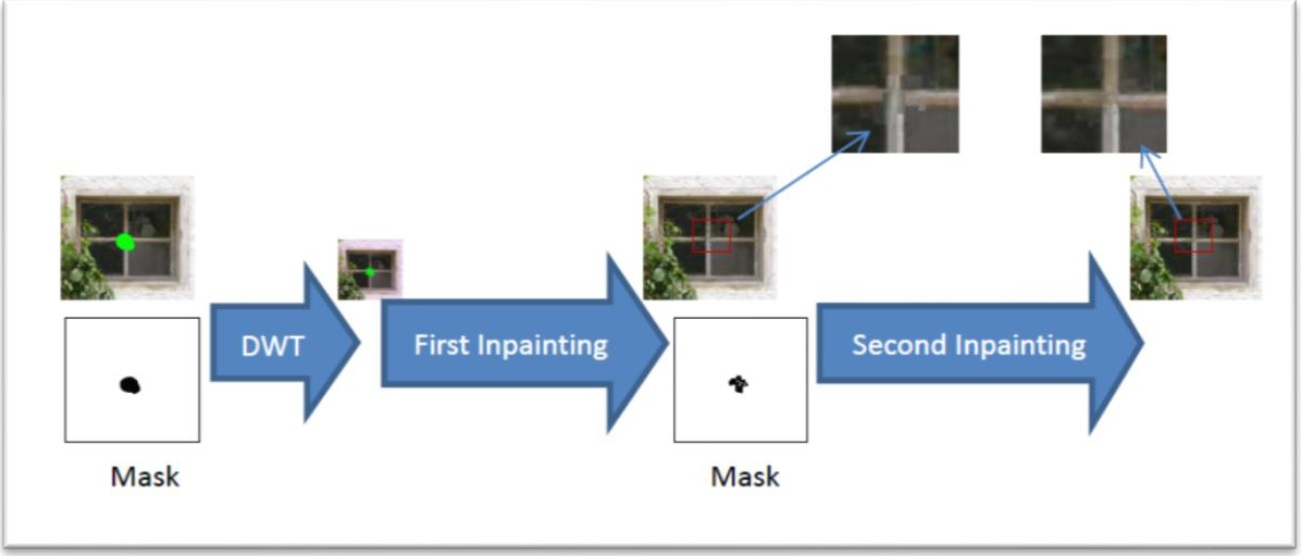
\includegraphics[width=0.9\textwidth]{ch4/fig5.eps}\\
(a)cars2 \quad\quad (b)car3 \quad\quad\quad (c)cars4 \quad\quad\quad (d)people1 \quad\quad (e)people2
% figure caption is below the figure
\end{center}
\caption{算法比较结果}
\label{ch4:fig:result}       % Give a unique label
\end{figure}

文献~\inlinecite{kwak2011Generalized,Multitransform}的结果来自于文献~\inlinecite{Multitransform},文献~\inlinecite{5.8s} 的源代码来自于作者的个人网站\footnote{https://sites.google.com/site/homekmyi/}。从图~\ref{ch4:fig:result}中可以看到,本文算法与文献~\inlinecite{Multitransform}算法提取的前景相对于文献\cite{kwak2011Generalized,5.8s}的结果 要更加准确。为了进行定量分析,使用提取的前景像素与正确值之间比较得到的精度、召回率以及F-Score指标来评估算法的有效性。其中精度$P$定义为:
$$ P = \frac{TP}{(TP+FP)}$$
召回率$R$定义为:
$$R = \frac{TP}{(TP+FN)}$$
F-Score定义为
$$F = \frac{2 \times P \times R}{(P + R)}$$
其中$TP,FP,FN,TN$分别为前景结果与正确前景比较后统计的正确前景像素数量,错误前景像素数量,错误背景像素数量以及正确背景像素数量。从定义可以看出,这三个指标的最大值均为1,且指标越高说明算法的准确度越好。表~\ref{ch4:tab:result1}中列出了本章算法与文献~\inlinecite{kwak2011Generalized,Multitransform,5.8s}算法在12个视频中得到的平均精度、召回率和F-Score值。从表~\ref{ch4:tab:result1}中可以看出,在大多数情况下,本章算法得到的前景准确度高于其他算法,并且本章算法在三个指标上均得到了最高的平均值。 在使用稀疏光流和基于超像素的MRF优化的情况下,本章算法的平均 F-Score值仍然比文献~\inlinecite{Multitransform}中基于稠密光流和像素级MRF的算法略高。\par

由于本章的算法基于运动线索和背景模型,当输入视频的第一帧图像中已经包含前景对象时,背景模型会在初始化时将前景标为背景。这会造成本章算法提取的前景结果在视频的前几帧包含一些错误的前景。随着本章算法继续运行,这些错误前景像素会随着背景模型更新以及包含运动线索的全局优化过程快速消失。当输入视频的第一帧不包含前景对象时,并不会存在上述的问题。在实验中对比时,忽略这类测试视频的前面几帧图像。由于本章算法的运动线索来自于SSRG算法,并假设可追踪的大部分特征点来自于背景。在自然环境中拍摄的大多数视频均满足这一假设,但是当视频中不满足这一假设时,例如行走的人的局部特写镜头,本章算法可能无法得到基于运动线索的粗略结果,从而造成算法无法得到准确的前景。\par


\begin{table}[htb]

% table caption is above the table
\caption{算法准确度比较,最好的结果用粗体表示}
\label{ch4:tab:result1}       % Give a unique label
% For LaTeX tables use
\resizebox{\textwidth}{!}{
\begin{tabular}{ccccccccccccc} \toprule[1.5pt]
\multicolumn{1}{c}{\multirow {2}{*}{}}&\multicolumn{3}{c}{本章算法}& \multicolumn{3}{c}{\inlinecite{Multitransform}算法}& \multicolumn{3}{c}{\inlinecite{kwak2011Generalized}算法}& \multicolumn{3}{c}{\inlinecite{5.8s}算法}\\
\cline{2-13}
\multicolumn{1}{c}{}&\multicolumn{1}{c}{P}&\multicolumn{1}{c}{R}&\multicolumn{1}{c}{F}&\multicolumn{1}{c}{P}&\multicolumn{1}{c}{R}&\multicolumn{1}{c}{F}&\multicolumn{1}{c}{P}&\multicolumn{1}{c}{R}&\multicolumn{1}{c}{F}&\multicolumn{1}{c}{P}&\multicolumn{1}{c}{R}&\multicolumn{1}{c}{F}\\
\hline
\multicolumn{1}{c}{vcar}&\multicolumn{1}{c}{\textbf{0.940}}&\multicolumn{1}{c}{\textbf{0.887}}&\multicolumn{1}{c}{\textbf{0.913}}&\multicolumn{1}{c}{0.839}&\multicolumn{1}{c}{0.856}&\multicolumn{1}{c}{0.846}&\multicolumn{1}{c}{0.595}&\multicolumn{1}{c}{0.626}&\multicolumn{1}{c}{0.607}&\multicolumn{1}{c}{0.690}&\multicolumn{1}{c}{0.365}&\multicolumn{1}{c}{0.478}\\
\multicolumn{1}{c}{vperson}&\multicolumn{1}{c}{0.757}&\multicolumn{1}{c}{0.898}&\multicolumn{1}{c}{0.821}&\multicolumn{1}{c}{\textbf{0.823}}&\multicolumn{1}{c}{\textbf{0.936}}&\multicolumn{1}{c}{\textbf{0.873}}&\multicolumn{1}{c}{0.539}&\multicolumn{1}{c}{0.628}&\multicolumn{1}{c}{0.568}&\multicolumn{1}{c}{0.753}&\multicolumn{1}{c}{0.476}&\multicolumn{1}{c}{0.583}\\
\multicolumn{1}{c}{cars1}&\multicolumn{1}{c}{0.757}&\multicolumn{1}{c}{\textbf{0.974}}&\multicolumn{1}{c}{\textbf{0.852}}&\multicolumn{1}{c}{0.729}&\multicolumn{1}{c}{0.945}&\multicolumn{1}{c}{0.822}&\multicolumn{1}{c}{\textbf{0.843}}&\multicolumn{1}{c}{0.738}&\multicolumn{1}{c}{0.785}&\multicolumn{1}{c}{0.527}&\multicolumn{1}{c}{0.379}&\multicolumn{1}{c}{0.441}\\
\multicolumn{1}{c}{cars2}&\multicolumn{1}{c}{\textbf{0.886}}&\multicolumn{1}{c}{\textbf{0.934}}&\multicolumn{1}{c}{\textbf{0.910}}&\multicolumn{1}{c}{0.698}&\multicolumn{1}{c}{0.908}&\multicolumn{1}{c}{0.789}&\multicolumn{1}{c}{0.679}&\multicolumn{1}{c}{0.741}&\multicolumn{1}{c}{0.705}&\multicolumn{1}{c}{0.282}&\multicolumn{1}{c}{0.131}&\multicolumn{1}{c}{0.179}\\
\multicolumn{1}{c}{cars3}&\multicolumn{1}{c}{\textbf{0.841}}&\multicolumn{1}{c}{\textbf{0.969}}&\multicolumn{1}{c}{\textbf{0.901}}&\multicolumn{1}{c}{0.820}&\multicolumn{1}{c}{0.956}&\multicolumn{1}{c}{0.882}&\multicolumn{1}{c}{0.804}&\multicolumn{1}{c}{0.802}&\multicolumn{1}{c}{0.802}&\multicolumn{1}{c}{0.505}&\multicolumn{1}{c}{0.236}&\multicolumn{1}{c}{0.322}\\
\multicolumn{1}{c}{cars4}&\multicolumn{1}{c}{\textbf{0.951}}&\multicolumn{1}{c}{\textbf{0.932}}&\multicolumn{1}{c}{\textbf{0.942}}&\multicolumn{1}{c}{0.877}&\multicolumn{1}{c}{0.917}&\multicolumn{1}{c}{0.895}&\multicolumn{1}{c}{0.575}&\multicolumn{1}{c}{0.679}&\multicolumn{1}{c}{0.621}&\multicolumn{1}{c}{0.502}&\multicolumn{1}{c}{0.251}&\multicolumn{1}{c}{0.335}\\
\multicolumn{1}{c}{cars5}&\multicolumn{1}{c}{\textbf{0.926}}&\multicolumn{1}{c}{0.777}&\multicolumn{1}{c}{0.845}&\multicolumn{1}{c}{0.892}&\multicolumn{1}{c}{\textbf{0.857}}&\multicolumn{1}{c}{\textbf{0.874}}&\multicolumn{1}{c}{0.623}&\multicolumn{1}{c}{0.680}&\multicolumn{1}{c}{0.645}&\multicolumn{1}{c}{0.659}&\multicolumn{1}{c}{0.138}&\multicolumn{1}{c}{0.228}\\
\multicolumn{1}{c}{cars6}&\multicolumn{1}{c}{0.866}&\multicolumn{1}{c}{\textbf{0.988}}&\multicolumn{1}{c}{\textbf{0.923}}&\multicolumn{1}{c}{\textbf{0.868}}&\multicolumn{1}{c}{0.942}&\multicolumn{1}{c}{0.903}&\multicolumn{1}{c}{0.624}&\multicolumn{1}{c}{0.890}&\multicolumn{1}{c}{0.731}&\multicolumn{1}{c}{0.584}&\multicolumn{1}{c}{0.140}&\multicolumn{1}{c}{0.226}\\
\multicolumn{1}{c}{cars7}&\multicolumn{1}{c}{0.714}&\multicolumn{1}{c}{\textbf{0.974}}&\multicolumn{1}{c}{0.824}&\multicolumn{1}{c}{\textbf{0.802}}&\multicolumn{1}{c}{0.950}&\multicolumn{1}{c}{\textbf{0.869}}&\multicolumn{1}{c}{0.662}&\multicolumn{1}{c}{0.729}&\multicolumn{1}{c}{0.691}&\multicolumn{1}{c}{0.282}&\multicolumn{1}{c}{0.311}&\multicolumn{1}{c}{0.296}\\
\multicolumn{1}{c}{cars8}&\multicolumn{1}{c}{\textbf{0.793}}&\multicolumn{1}{c}{\textbf{0.945}}&\multicolumn{1}{c}{\textbf{0.862}}&\multicolumn{1}{c}{0.737}&\multicolumn{1}{c}{0.944}&\multicolumn{1}{c}{0.826}&\multicolumn{1}{c}{0.775}&\multicolumn{1}{c}{0.766}&\multicolumn{1}{c}{0.767}&\multicolumn{1}{c}{0.529}&\multicolumn{1}{c}{0.699}&\multicolumn{1}{c}{0.602}\\
\multicolumn{1}{c}{people1}&\multicolumn{1}{c}{\textbf{0.947}}&\multicolumn{1}{c}{\textbf{0.879}}&\multicolumn{1}{c}{\textbf{0.912}}&\multicolumn{1}{c}{0.925}&\multicolumn{1}{c}{0.816}&\multicolumn{1}{c}{0.866}&\multicolumn{1}{c}{0.492}&\multicolumn{1}{c}{0.693}&\multicolumn{1}{c}{0.563}&\multicolumn{1}{c}{0.760}&\multicolumn{1}{c}{0.393}&\multicolumn{1}{c}{0.518}\\
\multicolumn{1}{c}{people2}&\multicolumn{1}{c}{\textbf{0.950}}&\multicolumn{1}{c}{\textbf{0.981}}&\multicolumn{1}{c}{\textbf{0.965}}&\multicolumn{1}{c}{0.939}&\multicolumn{1}{c}{0.895}&\multicolumn{1}{c}{0.916}&\multicolumn{1}{c}{0.850}&\multicolumn{1}{c}{0.774}&\multicolumn{1}{c}{0.808}&\multicolumn{1}{c}{0.728}&\multicolumn{1}{c}{0.425}&\multicolumn{1}{c}{0.537}\\
\hline
\multicolumn{1}{c}{平均}&\multicolumn{1}{c}{\textbf{0.860}}&\multicolumn{1}{c}{\textbf{0.928}}&\multicolumn{1}{c}{\textbf{0.889}}&\multicolumn{1}{c}{0.829}&\multicolumn{1}{c}{0.910}&\multicolumn{1}{c}{0.868}&\multicolumn{1}{c}{0.670}&\multicolumn{1}{c}{0.729}&\multicolumn{1}{c}{0.698}&\multicolumn{1}{c}{0.597}&\multicolumn{1}{c}{0.333}&\multicolumn{1}{c}{0.428}\\
\bottomrule[1.5pt]

\end{tabular}
}
\end{table}


\begin{table}
\caption{算法速度与准确度比较}
\begin{center}
\label{ch4:tab:result2}
\begin{tabular}{cccc}

  \toprule[1.5pt]
  % after \\: \hline or \cline{col1-col2} \cline{col3-col4} ...
  算法 & 预处理 & 速度(帧/秒) & F-Score \\
\hline
  \inlinecite{Multitransform}算法 & 稠密光流 & NA & 0.848 \\
  \inlinecite{gbsuperpixel}算法 & 稠密光流 & 0.17 & 0.923 \\
  \inlinecite{5.8s}算法 & 无  & 45& 0.419 \\
  本章算法 & 无 & 7.65 & 0.910 \\
  \bottomrule[1.5pt]

\end{tabular}
\end{center}
\end{table}

%\begin{table}
%\caption{Comparison of computation time}
%\label{tab:2}
%\begin{tabular}
%  \hline
%  % after \\: \hline or \cline{col1-col2} \cline{col3-col4} ...
%  Algorithm & Preprocessing & Speed & Accuracy \\
%  \cite{GbsSuperpixel} & Dense Optical Flow & 0.17fps & ? \\
%  \cite{SubspaceTracking} & Dense Point Trajectories & 0.55fps & ? \\
%  \cite{5.8s} & No  & 170fps & ? \\
%  ours & No & 20fps @320*240 & ? \\
%  \hline
%\end{tabular}
%\end{table}
% For one-column wide figures use
\begin{figure}[!htbp]
\begin{center}
% Use the relevant command to insert your figure file.
% For example, with the graphicx package use
  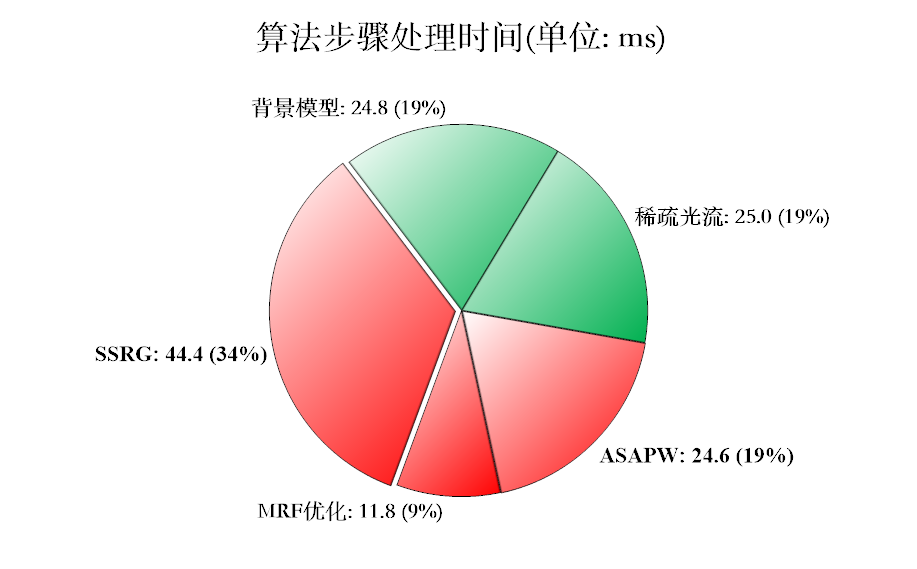
\includegraphics[width=0.8\textwidth]{ch4/timeing_chs.png}

% figure caption is below the figure
\end{center}

\caption{本章算法各步骤耗时,GPU实现步骤用绿色表示,视频大小为 $640\times480$}
\label{ch4:fig:timing}       % Give a unique label
\end{figure}
在算法速度方面,本章算法在处理大小为 640$\times$480 的视频时可以达到8帧/秒。在实验中,使用一台配备Intel i7 CPU和NVIDIA Geforce Titan GPU 的台式电脑。本章算法各步骤的耗时情况如图~\ref{ch4:fig:timing}所示,其中绿色标示的步骤为GPU实现。本章算法使用了OpenCV~\cite{opencv_library}中提供KLT算法的GPU版本,另外本章算法的背景模型部分也是通过CUDA~\cite{CUDA}在GPU上实现。从图~\ref{ch4:fig:timing}中可以看到,由于SSRG和MRF算法均在超像素上实现,这两步计算过程也较快。基于稀疏光流和SSRG算法,本章算法可以在70ms内获得基于运动线索的粗略前景结果。本章所提算法的速度与其他算法的比较情况如表\ref{ch4:tab:result2}所示。为了公平比较,表\ref{ch4:tab:result2}中列出了各算法在文献\inlinecite{HopKinsDataSet}中提供的四个视频(cars1, cars2, people1, people2)上得到的平均F-Score值。算法的速度和F-Score值均来自于各参考文献,其中文献~\inlinecite{Multitransform}中并没有介绍该算法的速度。这四个视频的原始大小为 $640\times480$。 与文献~\inlinecite{gbsuperpixel}算法相比,本章算法的速度大约是其 45 倍,而在精度上本章算法只比文献~\inlinecite{gbsuperpixel}算法稍差。文献\inlinecite{5.8s}所提出的算法非常快,但是其准确度与表\ref{ch4:tab:result2}中的其他算法相比差距较大,使得其无法应用于对前景检测准确度要求高的场合。此外,本章算法的一个重要优势是不需要计算稠密光流等预处理步骤,可以以即插即用的方式应用于很多准实时应用场景。
\subsection{实验二}
\label{ch4:sec:sub:test2}
在本小节中,将本章所提出算法在 CD.Net 2014数据集\cite{CD2014}进行了测试。首先,对数据集中的移动相机类视频进行了测试。在该分类中,有四个移动相机拍摄的长视频,其中包含的相机运动方式是旋转、平移和缩放(pan-tile-zoom, PTZ),四个视频的平均长度是2158帧。在实验中使用~\ref{ch4:sec:sub:test1}节中一样的参数设置。本章算法部分检测结果以及和其他算法的比较情况如图~\ref{ch4:fig:ptzResults}所示,其中第一列视频中相机连续水平方向旋转,第二列视频中相机断续旋转,第三列视频中相机在两个位置来回切换,第四列视频中相机连续缩放。从图~\ref{ch4:fig:ptzResults}中可以看出,本章算法可以处理相机的自由运动,特别在相机连续旋转(第一列)及缩放(第四列)时得到的前景结果明显好于其他算法。\par

\begin{figure}[htbp]
  \centering
  % Requires \usepackage{graphicx}
  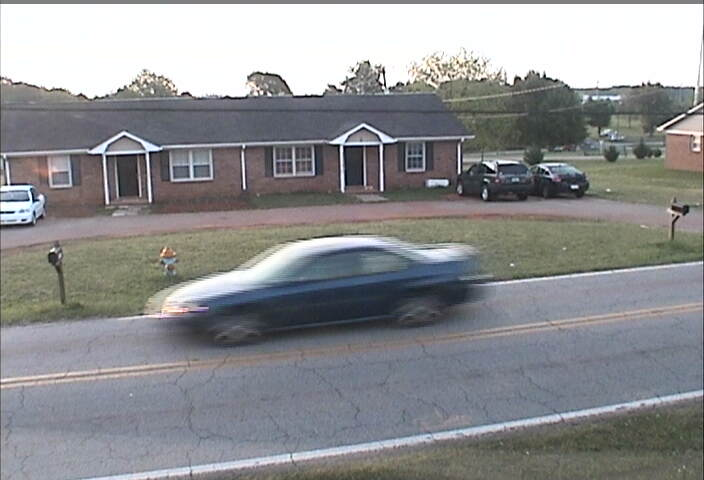
\includegraphics[width=0.22\textwidth,height=0.8in]{ch4/ptz/in000852.jpg}
  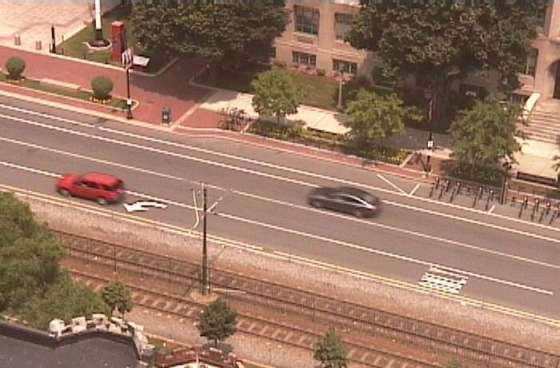
\includegraphics[width=0.22\textwidth,height=0.8in]{ch4/ptz/in002272.jpg}
  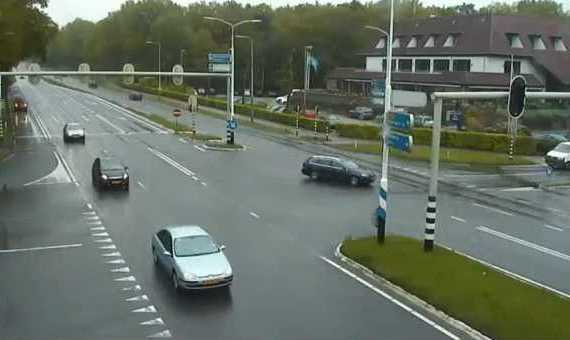
\includegraphics[width=0.22\textwidth,height=0.8in]{ch4/ptz/in001515.jpg}
  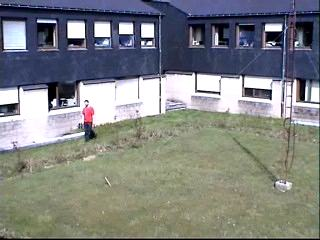
\includegraphics[width=0.22\textwidth,height=0.8in]{ch4/ptz/in000505.jpg}\\
  (a) 输入视频图像帧\\
  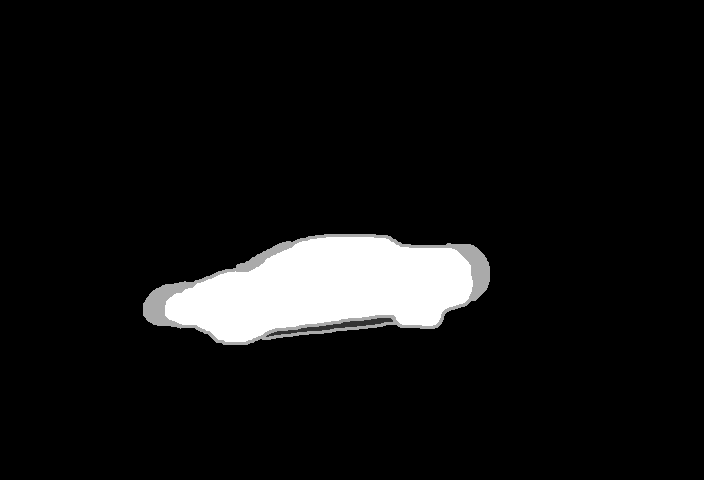
\includegraphics[width=0.22\textwidth,height=0.8in]{ch4/ptz/gt000852.png}
  \includegraphics[width=0.22\textwidth,height=0.8in]{ch4/ptz/gt002272.png}
  \includegraphics[width=0.22\textwidth,height=0.8in]{ch4/ptz/gt001515.png}
  \includegraphics[width=0.22\textwidth,height=0.8in]{ch4/ptz/gt000505.png}\\
  (b) 正确结果\\
  \includegraphics[width=0.22\textwidth,height=0.8in]{ch4/ptz/000852_ours.jpg}
  \includegraphics[width=0.22\textwidth,height=0.8in]{ch4/ptz/002272_ours.jpg}
  \includegraphics[width=0.22\textwidth,height=0.8in]{ch4/ptz/001515_ours.jpg}
  \includegraphics[width=0.22\textwidth,height=0.8in]{ch4/ptz/000505_ours.jpg}\\
  (c)本章算法结果\\
  \includegraphics[width=0.22\textwidth,height=0.8in]{ch4/ptz/000852_subsense.jpg}
  \includegraphics[width=0.22\textwidth,height=0.8in]{ch4/ptz/002272_subsense.jpg}
  \includegraphics[width=0.22\textwidth,height=0.8in]{ch4/ptz/001515_subsense.jpg}
  \includegraphics[width=0.22\textwidth,height=0.8in]{ch4/ptz/000505_subsense.jpg}\\
  (d)文献~\inlinecite{subsenseTIP}算法结果\\
  \includegraphics[width=0.22\textwidth,height=0.8in]{ch4/ptz/000852_pawcs.jpg}
  \includegraphics[width=0.22\textwidth,height=0.8in]{ch4/ptz/002272_pawcs.jpg}
  \includegraphics[width=0.22\textwidth,height=0.8in]{ch4/ptz/001515_pawcs.jpg}
  \includegraphics[width=0.22\textwidth,height=0.8in]{ch4/ptz/000505_pawcs.jpg}\\
  (e)文献~\inlinecite{Stcharles2015A}算法结果\\
  \includegraphics[width=0.22\textwidth,height=0.8in]{ch4/ptz/000852_sharedmodel.jpg}
  \includegraphics[width=0.22\textwidth,height=0.8in]{ch4/ptz/002272_sharedmodel.jpg}
  \includegraphics[width=0.22\textwidth,height=0.8in]{ch4/ptz/001515_sharedmodel.jpg}
  \includegraphics[width=0.22\textwidth,height=0.8in]{ch4/ptz/000505_sharedmodel.jpg}\\
  (f)文献~\inlinecite{Chen2015Learning}算法结果\\
  \includegraphics[width=0.22\textwidth,height=0.8in]{ch4/ptz/000852_cwisardh.jpg}
  \includegraphics[width=0.22\textwidth,height=0.8in]{ch4/ptz/002272_cwisardh.jpg}
  \includegraphics[width=0.22\textwidth,height=0.8in]{ch4/ptz/001515_cwisardh.jpg}
  \includegraphics[width=0.22\textwidth,height=0.8in]{ch4/ptz/000505_cwisardh.jpg}\\
  (g)文献~\inlinecite{Gregorio2014Change}算法结果\\
  \caption{CD.Net 2014数据集\cite{CD2014}PTZ分类视频检测结果比较}\label{ch4:fig:ptzResults}
\end{figure} \par

在算法定量分析中,使用了与文献~\cite{CD2014}一致的指标。此外,为了比较提取前景的准确度,计算提取前景图像与正确值之间的峰值信噪比(peak signal noise ratio, PSNR),以及归一化互相关系数(normalized cross-correlation, NCC)。其中PSNR的计算方法为:
 $$MSE=\frac{1}{M\times N}\sum_{x,y}\left \| I_{x,y}-J_{x,y} \right \|^{2},PSNR = 20\times \log_{10}\left ( \frac{255}{\sqrt{MSE}}\right )$$
 NCC的计算方法为:
$$NCC=\frac{\sum_{x,y}\left( I_{x,y}-\bar J_{x,y}\right )\left(J_{x,y}- \bar I_{x,y} \right )}{M\times N\times Std(I) \times Std(J)}$$
 其中$M$ 和 $N$分别为图像的宽度和高度。 $\bar I_{x,y},\bar J_{x,y}$ 分别表示图像$I$ and $J$ 的颜色均值,$Std$ 表示计算标准差。\par
 在图~\ref{ch4:fig:nccPSNR}中,将本章提出的算法(FMCBS),与文献~\inlinecite{Stcharles2015A}算法(PAWCS),文献\inlinecite{Chen2015Learning}算法(SharedModel),文献~\inlinecite{subsenseTIP}算法(SuBSENSE) 以及文献~\inlinecite{Gregorio2014Change}算法(CwisarDH)的NCC值和PSNR值进行了比较,各算法的NCC和PSNR值均为在四个视频得到的平均值,从在图~\ref{ch4:fig:nccPSNR}中可以看出,本章算法在这两个指标上均优于其他算法。
\begin{figure}[htb]
  \centering%
  \subcaptionbox{算法NCC比较} %标题的长度,超过则会换行,如下一个小图。
    {\includegraphics[width=0.45\textwidth]{ch4/ncc.png}}%
 \hspace{1em}%
  \subcaptionbox{算法PSNR比较}
      {\includegraphics[width=0.45\textwidth]{ch4/psnr.png}}

  \caption{算法NCC和PSNR比较结果}
  \label{ch4:fig:nccPSNR}
\end{figure}


 在表~\ref{ch4:tab:resultPTZ}中列出了本章算法的到的平均结果以及与其他领先的算法比较的结果。通过比较,在本文完成时本章算法在CD.Net 2014数据集\cite{CD2014} 的PTZ 类别中综合排名第一\footnote{见 http://wordpress-jodoin.dmi.usherb.ca/results2014/412/}。该综合排名是计算算法在7 项指标中的综合排名得到的。这7项指标除了~\ref{ch4:sec:sub:test1}节中使用的精度(P)、召回率(R)、F-Score(F)之外,还包括敏感度(specificity, Sp)、错误前景率(false positive rate, FPR)、错误背景率(false negative rate, FNR)以及错误分类百分比(percentage of wrong classifications, PWC),这些指标的定义为:
 $$ Sp = \frac{TN}{(TN + FP)},FPR = \frac{FP}{(FP+TN)}, FNR = \frac{FN}{(TP+FN)} $$
 $$ PWC = 100 \times \frac{(FN+FP)}{(TP+FN+FP+TN)} $$
 其中FPR、FNR、PWC均表示错误概率,值越小表示算法越好,其他指标均越大越好。
 \begin{table}[ht]
\caption{CD.Net 2014数据集\cite{CD2014}中的PTZ分类视频处理结果比较}
\label{ch4:tab:resultPTZ}
\resizebox{\textwidth}{!}{
\begin{tabular}{ccccccccc} %% this creates two columns
%% |l|l| to left justify each column entry
%% |c|c| to center each column entry
%% use of \rule[]{}{} below opens up each row
\toprule[1.5pt]
\rule[-1ex]{0pt}{3.5ex}  算法 & 排名 & R &Sp & FPR & FNR &PWC &F &P  \\
\hline
\rule[-1ex]{0pt}{3.5ex}  FMCBS & 3.86 & 0.834 & 0.998 & 0.003 & 0.167 &0.384&0.704&0.645 \\

\rule[-1ex]{0pt}{3.5ex}  PAWCS\cite{Stcharles2015A}&9.43&0.698&0.991&0.009&0.302&1.116&0.461&0.473 \\

\rule[-1ex]{0pt}{3.5ex}  SharedModel\cite{Chen2015Learning}&  11.71&0.797&0.979&0.021&0.203&2.217&0.386&0.312  \\

\rule[-1ex]{0pt}{3.5ex}  SuBSENSE\cite{subsenseTIP}&  13.43&0.831&0.963&0.037&0.169&3.816&0.348&0.284 \\

\rule[-1ex]{0pt}{3.5ex}  CwisarDH\cite{Gregorio2014Change}&13.57&0.336&0.998&0.002&0.664&0.685&0.322&0.482  \\
\bottomrule[1.5pt]
\end{tabular}}
\end{table}

%\begin{table}[ht]
%\caption{CD.Net 2014数据集\cite{CD2014}中的PTZ分类视频处理结果比较}
%\label{ch4:tab:resultPTZ}
%\resizebox{\textwidth}{!}{
%\begin{tabular}{ccccccccccc} %% this creates two columns
%%% |l|l| to left justify each column entry
%%% |c|c| to center each column entry
%%% use of \rule[]{}{} below opens up each row
%\toprule[1.5pt]
%\rule[-1ex]{0pt}{3.5ex}  算法 & 排名 & R &Sp & FPR & FNR &PWC &F &P & NCC & PSNR \\
%\hline
%\rule[-1ex]{0pt}{3.5ex}  FMCBS & 3.86 & 0.834 & 0.998 & 0.003 & 0.167 &0.384&0.704&0.645 &0.194&27.654\\
%
%\rule[-1ex]{0pt}{3.5ex}  PAWCS\cite{Stcharles2015A}&9.43&0.698&0.991&0.009&0.302&1.116&0.461&0.473&0.155&17.657 \\
%
%\rule[-1ex]{0pt}{3.5ex}  SharedModel\cite{Chen2015Learning}&  11.71&0.797&0.979&0.021&0.203&2.217&0.386&0.312&0.174&12.392  \\
%
%\rule[-1ex]{0pt}{3.5ex}  SuBSENSE\cite{subsenseTIP}&  13.43&0.831&0.963&0.037&0.169&3.816&0.348&0.284&0.193&15.992 \\
%
%\rule[-1ex]{0pt}{3.5ex}  CwisarDH\cite{Gregorio2014Change}&13.57&0.336&0.998&0.002&0.664&0.685&0.322&0.482&0.105&18.708  \\
%\bottomrule[1.5pt]
%\end{tabular}}
%\end{table}


为了测试本章算法的可扩展性,将本章算法的参数进行调整后在CD.Net 2014数据库中的静态相机情况下动态背景类中两个较困难的视频(boats,canoe)上进行了测试。由于测试视频中摄像机是固定的,这时本章算法的运动线索无效,因此在此实验中所用的背景模型中以文献~\inlinecite{subsenseTIP}中定义的更新机制对背景模型进行更新,只用基于外观模型的线索来处理静态相机视频。本章算法得到的部分结果以及和其他算法的比较情况如图~\ref{ch4:fig:dbresults}所示,其中图~\ref{ch4:fig:dbresults}(a)和(f)中为输入视频的一帧图像,从图中看出图像中包含的水面部分的波纹和浪花属于动态背景。从图~\ref{ch4:fig:dbresults}中的处理结果可以看到,本章算法和其他基于采样模型的算法\cite{pbas,subsenseTIP}均能较好的处理动态背景,没有将水面部分误识别为前景,此外本章算法得到的前景准确度要优于文献~\inlinecite{subsenseTIP}算法得到的结果。在表~\ref{ch4:tab:resultsDB}中列出了本章算法的结果以及同其他基于采样模型的算法的比较。由于文献~\inlinecite{Chien2002Efficient}中的算法只有一张图像类背景建模,使得该算法无法有效处理包含动态背景的视频。各算法得到前景结果的定量分析和比较如表~\ref{ch4:tab:resultsDB}所示。从表~\ref{ch4:tab:resultsDB}中可以看出,本章所提出的算法得到的精度指标F-Score好于原来的SuBSENSE算法\cite{subsenseTIP},这主要得益于本章算法的MRF优化算法。
\begin{figure}
  \centering
  % Requires \usepackage{graphicx}
  \includegraphics[width=0.19\textwidth]{ch4/db/boat.jpg}
  \includegraphics[width=0.19\textwidth]{ch4/db/boat_gt.jpg}
  \includegraphics[width=0.19\textwidth]{ch4/db/boat_MCBS.jpg}
  \includegraphics[width=0.19\textwidth]{ch4/db/boat_pbas_23.jpg}
  \includegraphics[width=0.19\textwidth]{ch4/db/boat_Pierre_LucSt_CharlesJul2014_139.jpg}\\
  (a)boats视频帧(b)正确结果(c)本章算法结果(d)~\inlinecite{pbas}算法结果(e)\inlinecite{subsenseTIP}算法结果 \\
  \includegraphics[width=0.19\textwidth]{ch4/db/canoe.jpg}
  \includegraphics[width=0.19\textwidth]{ch4/db/canoe_gt.png}
  \includegraphics[width=0.19\textwidth]{ch4/db/canoe_MCBS.jpg}
  \includegraphics[width=0.19\textwidth]{ch4/db/canoe_pbas_23.jpg}
  \includegraphics[width=0.19\textwidth]{ch4/db/canoe_Pierre_LucSt_CharlesJul2014_139.jpg}\\
  (f)canoe视频帧(g)正确结果(h)本章算法结果(i)~\inlinecite{pbas}算法结果(j)\inlinecite{subsenseTIP}算法结果 \\
  \caption{CD.Net 2014\cite{CD2014} 数据集动态背景分类中的 boats 和 canoe视频处理结果对比}\label{ch4:fig:dbresults}
\end{figure}


 \begin{table}[ht]
\caption{CD.Net 2014 数据集\cite{CD2014}动态背景分类的 boats 和 canoe视频处理结果精度比较}
\label{ch4:tab:resultsDB}
\begin{center}
\begin{tabular}{cccccccc} %% this creates two columns
%% |l|l| to left justify each column entry
%% |c|c| to center each column entry
%% use of \rule[]{}{} below opens up each row
\toprule[1.5pt]
\rule[-1ex]{0pt}{3.5ex}  算法 &R &Sp & FPR & FNR &PWC &F &P\\
\hline
\rule[-1ex]{0pt}{3.5ex}  EMOS\cite{Chien2002Efficient}&  0.240&0.987&0.013&0.760&1.993&0.184&0.150 \\

\rule[-1ex]{0pt}{3.5ex}  PBAS\cite{pbas}&0.359&1.000&0.000&0.641&0.604&0.527&0.992  \\

\rule[-1ex]{0pt}{3.5ex}  SuBSENSE\cite{subsenseTIP}&  0.600&1.000&0.000&0.400&0.408&0.734&0.945 \\

\rule[-1ex]{0pt}{3.5ex}  FMCBS &  0.734 & 0.999 & 0.001 & 0.257 &0.319&0.814&0.899\\

\rule[-1ex]{0pt}{3.5ex}  PAWCS\cite{Stcharles2015A}&0.844&0.999&0.001&0.156&0.211&0.882&0.924\\
\bottomrule[1.5pt]
\end{tabular}
\end{center}
\end{table}


 \section{本章小结}
 \label{ch4:sec:conclusions}
 视频背景减除技术的目的是将视频图像序列中的背景部分与前景部分分离,从而提取准确的前景对象。在视频中,一般认为前景是相对运动的对象,而背景为相对静止的对象。当拍摄视频的相机自身包含旋转、平移、缩放等自由运动时,从其所拍摄的视频中提取准确的前景会更加困难。本章研究了针对移动相机的视频减除算法,针对目前已有算法需要进行稠密光流或像素点轨迹预处理过程,算法耗时严重的问题,本章提出了一种快速准确的视频背景减除算法。\par
 本章所提出的算法主要依靠两类线索来有效检测自由移动相机所拍摄视频中的前景对象。首先,利用基于采样的背景模型获取基于外观的线索。为了估算并补偿相机的运动,本章算法引入了ASAPW技术,通过图像不同区域的多个单应性矩阵来估算相机运动。与传统的全局单应性矩阵方法相比,ASAPW方法通用性更强,可以处理任何情况下的相机运动,且准确度高。本章算法中对原有的ASAPW算法~\cite{Liu_2013ASAP}进行了改进,提高了求解的速度。将经ASAPW处理后的图像与背景模型的匹配结果,可以获得基于外观线索的粗略前景结果;在另一方面,由于前景对象的运动和相机的运动不同,利用这一基于运动的线索可以获得另一个粗略的前景结果。与之前的算法不同,本章算法没有利用稠密光流或像素点轨迹的方法来处理前景对象的运动情况。为了加快速度,本章算法利用效率更高的稀疏点光流来获得基于超像素的光流场。通过与相机运动情况的比较,将一部分运动情况与相机运动十分接近的超像素标记为背景种子点,随后通过SSRG算法将这些稀疏的背景种子点扩散到整幅图像,从而获得基于运动线索的粗略前景结果;最后,综合考虑两类线索,以及相邻视频图像帧之间的连续性,通过基于超像素的MRF优化方法建立能量函数并利用图割算法求解能量最小化问题获得最终的前景结果。\par
 本章算法中的一些步骤,例如背景模型匹配与更新,稀疏点光流等均通过CUDA在GPU上实现并行处理,进一步提高了本章算法的速度。实验结果证明,本章算法提取前景的准确度与先进算法的水平相当,但是在速度上和易用性上却有较大优势。本章算法处理大小为 $640\times480$的视频可以达到8帧/秒的速度,对于分辨率更低$320\times240$的视频可以实现实时处理。然而随着摄影设备的发展,目前主流的手机、摄像机等拍摄视频分辨率远超过实验中所用视频,因此需要在保证准确度的同时进一步提高算法的速度。
